\subsection{Dynamic Reasoning Paradigm during Inference}
\label{sec:dynamic}

Existing works focus on \textit{modifying the reasoning paradigm} for more efficient inference. The key during inference is choosing the proper criterion to guide the reasoning strategy. Current training-free approaches explore dynamic reasoning using various criteria, such as reward-guided, confidence-based, and consistency-based selective reasoning. Additionally, a summarization-based dynamic reasoning method intrinsically integrates the output summarization paradigm of LLMs during training.

\insightbox{The key question is: Which criterion to guide the inference? What is the appropriate efficient inference paradigm?}

\begin{table}[htbp]
\centering
% \resizebox{\textwidth}{!}{
\scriptsize
% \begin{tabularx}{\textwidth}{XXXXX}
\caption{Comparison of different methods of dynamic reasoning paradigm of test time compute during inference.}
\scalebox{0.99}{
\begin{tabular}{p{1.5cm} p{2cm} p{0.8cm} p{3cm} p{4cm}}
\toprule
\textbf{Category} & \textbf{Method} & \textbf{Training-free?} & \textbf{Baseline and Its Drawbacks} & \textbf{Method Description} \\ \midrule
\multirow{2}{*}{\parbox{1.7cm}{Reward-guided Efficient Reasoning}} 
  & Speculative Rejection~\cite{sun2024fast} & Yes & \textbf{Best-of-N (BoN) Decoding}: underutilizes GPU memory and computational resources during the early stages, leading to lower final rewards. & Starts BoN with a large initial batch size and rejects unpromising sequences periodically, efficiently achieving higher rewards. \\ 
  \cmidrule(l){2-5}
  & Reward-Guided Speculative Decoding (RSD) \cite{liao2025reward} & Yes & \textbf{Speculative Decoding}: strictly enforces unbiasedness, discarding useful intermediate outputs and leading to computational inefficiency. & A speculative decoding method that leverages a reward model (PRM) to selectively accept high-quality outputs from a lightweight draft model, reducing computation while preserving accuracy. \\
  \midrule
  \multirow{4}{*}{\parbox{1.7cm}{Confidence/ Certainty-based Adaptive Reasoning}} & Dynamic Parallel Tree Search \cite{ding2025dynamic} & Yes & \textbf{Tree-of-Thoughts:} difficult to parallelize due to frequent switching of reasoning focus, and inefficient because of redundant exploration of suboptimal solutions & Dynamically parallelizes node expansion through adaptive batching and implements a search-and-transition mechanism (including \textit{Early Stop} and \textit{Deep Seek}) to prune unpromising paths early. \\
  \cmidrule(l){2-5}
  & Dynasor (Certaindex-based Scheduling) \cite{fu2024efficiently} & Yes & \textbf{Serving systems with uniform resource allocation}: allocate compute uniformly, leading to inefficient resource usage and unmet latency targets & Dynamically allocates compute for reasoning queries based on \textit{Certaindex}, a statistical measure of reasoning progress, to maximize accuracy within resource constraints. \\ 
  \cmidrule(l){2-5}
  & FastMCTS \cite{li2025fastmcts} & Yes & \textbf{Rejection Sampling}: inefficient, discards intermediate steps, and fails to balance problem difficulty & An MCTS-inspired sampling strategy that efficiently generates high-quality multi-step reasoning data, providing step-level evaluation signals and balanced sampling across problem difficulties. \\ 
  \cmidrule(l){2-5}
  & Length-filtered Vote \cite{wu2025more} & Yes & \textbf{Majority Voting}: ignores reasoning quality, includes suboptimal CoT lengths, and suffers from noisy predictions & A voting strategy that selects answers with the optimal CoT length by filtering out excessively short or long reasoning paths. \\
  \midrule
  Consistency-based Selective Reasoning & Self-Truncation Best-of-N (ST-BoN) \cite{wang2025sampling} & Yes & \textbf{Best-of-N Sampling}: fully generates all samples and relies on costly reward models & Estimates the most promising sample early via internal embedding consistency, truncating inferior samples prematurely. \\
  \midrule
  \multirow{2}{*}{\parbox{1.7cm}{Summarization-based Dynamic Reasoning}} & LightThinker \cite{zhang2025lightthinker} & No & \textbf{Chain-of-Thought (CoT)}: high memory and computational overhead due to the generation of an excessive number of tokens & Trains LLMs to learn when and how to compress intermediate thoughts, condensing long reasoning chains into gist tokens, and uses a sparse-patterned attention mask during inference to enhance computational efficiency. \\
    \cmidrule(l){2-5}
  & InftyThink \cite{yan2025inftythink} & No & \textbf{Monolithic Reasoning}: reasoning output is verbose, and can quickly exceed the context window limit of the LLM, resulting in poor performance & An iterative reasoning paradigm that interleaves reasoning steps with intermediate summarization, enabling unbounded reasoning depth without architectural modifications. \\
\bottomrule
\end{tabular}
}
\end{table}

\subsubsection{Dynamic Reasoning via Explicit Criteria}

Train-time scaling with RL~\cite{guo2025deepseek} can significantly enhance the reasoning ability of LLMs. However, it requires substantial computational resources to scale up the model training, making it prohibitively expensive~\cite{guo2025deepseek}.
As an alternative, researchers have explored test-time reasoning, also known as test-time scaling~\cite{snell2024scaling}. Instead of relying on training to learn CoT reasoning steps, test-time scaling leverages various inference strategies that allow models to ``think longer and broader'' on complex problems. This approach consistently improves performance on challenging math and code problems that require reasoning by increasing the computational resources allocated during inference~\cite{snell2024scaling, beeching2024scalingtesttimecompute}.

Test-time scaling utilizes various inference strategies to generate longer and higher-quality CoT responses. There are several ways to scale up the inference. (1) Best-of-N sampling~\cite{sun2024fast, wang2025sampling} involves generating multiple responses for a given prompt, expanding the search space to identify better solutions. After generation, the best response is selected using either majority voting, where the most frequently occurring response is chosen; or by a reward model, which evaluates response quality based on pre-defined criteria. This method has been shown to significantly enhance the reasoning capabilities of LLMs~\cite{beeching2024scalingtesttimecompute}. (2) Beam-based searching~\cite{ding2025dynamic, fu2024efficiently,beeching2024scalingtesttimecompute}, which differs from Best-of-N by structuring generation into multiple steps. Instead of generating an entire response in one pass, beam search selects the most promising intermediate outputs with process reward model~\cite{uesato2022solving} at each step, while discarding less the optimal ones. This enables a more fine-grained optimization of both response generation and evaluation. (3) Monte Carlo Tree Search (MCTS)~\cite{li2025fastmcts}, where multiple solution paths are explored in parallel. MCTS generates partial responses along different branches of a solution tree, evaluates them, and back-propagates reward values to earlier nodes. The model then selects the branch with the highest cumulative reward, ensuring a more refined selection process compared to traditional beam search.

Although test-time scaling can significantly reduce train-time scaling up overhead~\cite{beeching2024scalingtesttimecompute}, the large number of generated responses still makes inference computationally expensive. To address this, recent works have been exploring methods to optimize test-time scaling.

\paragraph{Reward-guided Efficient Reasoning.}
%
Speculative Rejection~\cite{sun2024fast} is an efficient inference-time reasoning algorithm that optimizes Best-of-N (BoN) decoding by dynamically reducing computational overhead (as shown in Figure~\ref{fig:bonsample}, left). It generates multiple responses until memory limits are nearly reached, then \textit{discards low-quality outputs based on evaluation by a reward model}. This adaptive filtering substantially reduces inference costs compared to vanilla BoN.
%
On the other hand, Reward-Guided Speculative Decoding (RSD) \cite{liao2025reward} enhances the efficiency of speculative decoding specifically for multi-step reasoning tasks. Unlike traditional speculative decoding methods, which strictly require exact token matching between the draft model and target model, \textit{RSD leverages a Process Reward Model (PRM) to dynamically evaluate intermediate outputs} from the smaller, more efficient draft model. Outputs with high reward scores are directly accepted, while those with lower scores are further refined by a larger, more capable target model.

\paragraph{Confidence/Certainty-based Adaptive Reasoning.}
%
Dynamic Parallel Tree Search (DPTS)~\cite{ding2025dynamic} optimizes tree-based reasoning in LLMs by addressing two main inefficiencies by introducing: (1) \textit{Parallelism Streamline} optimizes memory and compute by storing only incremental KV cache updates and dynamically adjusting the number of extended nodes based on available GPU memory, (2) \textit{Search and Transition Mechanism} balances exploration and exploitation using confidence-based criteria. Overall, during inference, the system cuts off uncertain paths to save time.
%
FastMCTS~\cite{li2025fastmcts} is another confidence-based method that aims to optimize multi-step reasoning data synthesis. Traditional rejection sampling generates multiple candidate responses independently, selecting only the correct ones, but it is often inefficient and struggles with imbalanced sampling. Inspired by MCTS, FastMCTS prioritizes high-confidence traces for deep reasoning. Additionally, it adjusts tree expansion based on problem complexity, improving both efficiency and reasoning diversity.
%
Another line of research leverages certainty or uncertainty measures to guide adaptive reasoning. Certaindex~\cite{fu2024efficiently}, a certainty metric, quantifies the confidence of LLMs throughout reasoning using semantic entropy, reward model scores, or a combination of both. A higher certaindex indicates that further reasoning steps are unlikely to change the final answer, allowing early termination to free resources for more challenging queries. Dynasor, an inference system built on this principle, optimizes compute scheduling by dynamically tracking reasoning progress instead of allocating resources uniformly. Dynasor-CoT~\cite{fu2025reasoning} uses a probing scheme to exit early if the model is confident enough.
%
Length-filtered Vote~\cite{wu2025more} is another work that leverages uncertainty to improve CoT reasoning. The study finds that longer reasoning chains do not always improve accuracy; instead, performance initially improves but eventually declines due to error accumulation. The authors provide a mathematical analysis proving the existence of an optimal CoT length, determined by model capability and task difficulty. To exploit this, they propose Length-filtered Voting, a length-aware majority voting method that groups answers by CoT length and selects the most reliable group based on prediction uncertainty.
%
Self-Calib~\cite{huang2025efficient} introduces confidence-driven adaptive scaling strategies at test time to efficiently address queries with differing complexity levels, including Early-Stopping mechanisms for Best-of-N sampling and confidence-calibrated Self-Consistency approaches.
% 
CISC~\cite{taubenfeld2025confidence} implements a weighted majority voting scheme utilizing model-derived confidence scores. By emphasizing reasoning paths with higher confidence, it efficiently determines the correct response with substantially fewer samples. 

\paragraph{Consistency-based Selective Reasoning.} Self-Truncation Best-of-N (ST-BoN)~\cite{wang2025sampling} enhances BoN sampling efficiency by introducing early termination (as shown in Figure~\ref{fig:bonsample}, right), similar to Speculative Rejection~\cite{sun2024fast}. However, unlike Speculative Rejection using reward models, ST-BoN leverages consistency as the metric to measure the importance. Specifically, it leverages the consistency of latent embeddings to evaluate response quality. The core insight is that ``the closer a sample is to others, the more likely its path will lead to the correct answer''. Then, ST-BoN selects the most consistent Chain-of-Embedding (CoE) to others and regards it as the optimal sample.

\begin{figure}[t]
    \centering
    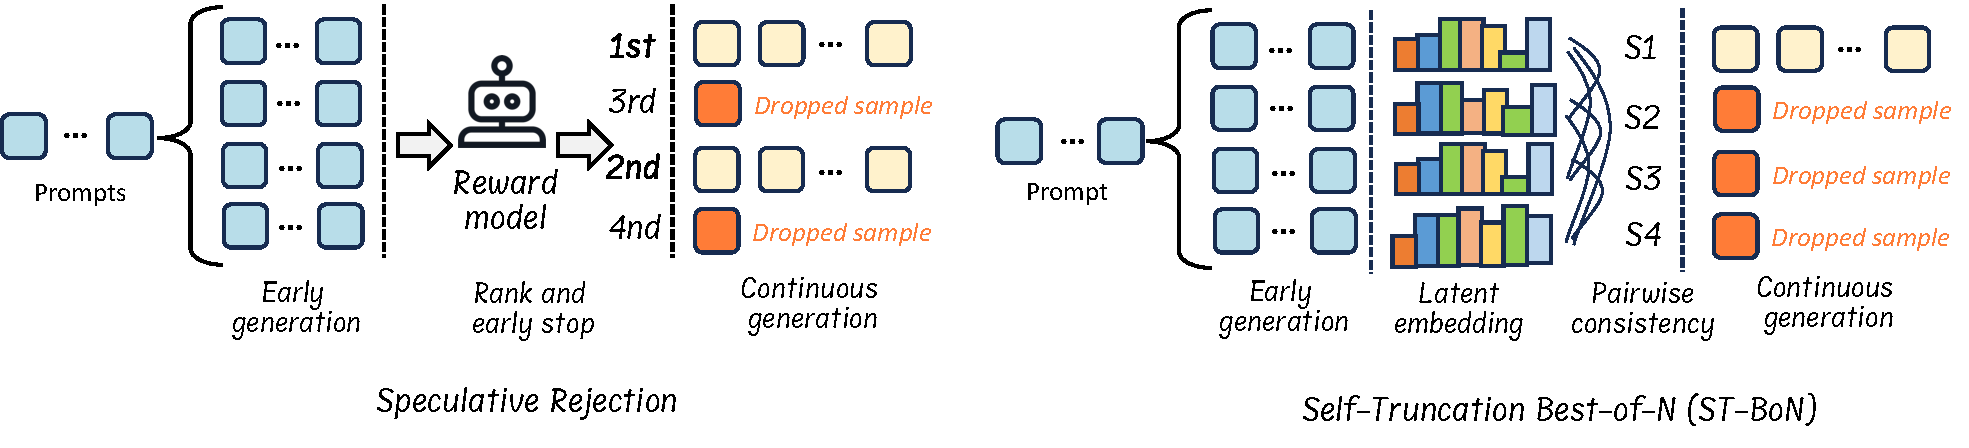
\includegraphics[width=\linewidth]{figs/testtimecompute.pdf}
    \caption{Examples of efficient Best-of-N sampling methods. \textit{(Left) Speculative Rejection}~\cite{sun2024fast} uses a reward model to estimate partial generation quality. It then early stops the sampled sequence with lower scores. \textit{(Right) ST-BoN}~\cite{wang2025sampling} evaluates the latent embedding of the early generation. The latent embedding of each thinking path will be used to calculate pairwise consistency between other tokens. The sequence with the highest consistency is more likely to arrive at the correct answer.}
    \label{fig:bonsample}
\end{figure}

\subsubsection{Summarization-based Dynamic Reasoning}

Some existing methods choose to optimize reasoning efficiency by training LLMs to \textit{summarize intermediate thinking steps}.
%
LightThinker \cite{zhang2025lightthinker} proposes to train LLMs to learn when and how to compress intermediate reasoning steps. Instead of storing long thought chains, LightThinker compresses verbose reasoning into compact ``gist tokens'' to reduce memory and computational costs. Implementing this summarization paradigm requires a sparse-patterned attention mask, ensuring the model focuses only on essential compressed representations. 
%
InftyThink \cite{yan2025inftythink} introduces an iterative reasoning method that enables essentially infinite reasoning chains while maintaining strong accuracy without surpassing the context window limit. It achieves this by iteratively generating a thought, summarizing it, and discarding previous thoughts and summaries, retaining only the most recent summary. Additionally, InftyThink provides a technique for converting existing reasoning datasets into an iterative format for training models under this paradigm. 






